%% This file was auto-generated by IPython.
%% Conversion from the original notebook file:
%% kmeans.ipynb
%%
\documentclass[11pt,english,fleqn]{article}

%% This is the automatic preamble used by IPython.  Note that it does *not*
%% include a documentclass declaration, that is added at runtime to the overall
%% document.

\usepackage{amsmath}
\usepackage{amssymb}
\usepackage{graphicx}
\usepackage{ucs}
\usepackage[utf8x]{inputenc}

% needed for markdown enumerations to work
\usepackage{enumerate}

% Slightly bigger margins than the latex defaults
\usepackage{geometry}
\geometry{verbose,tmargin=3cm,bmargin=3cm,lmargin=2.5cm,rmargin=2.5cm}

% Define a few colors for use in code, links and cell shading
\usepackage{color}
\definecolor{orange}{cmyk}{0,0.4,0.8,0.2}
\definecolor{darkorange}{rgb}{.71,0.21,0.01}
\definecolor{darkgreen}{rgb}{.12,.54,.11}
\definecolor{myteal}{rgb}{.26, .44, .56}
\definecolor{gray}{gray}{0.45}
\definecolor{lightgray}{gray}{.95}
\definecolor{mediumgray}{gray}{.8}
\definecolor{inputbackground}{rgb}{.95, .95, .85}
\definecolor{outputbackground}{rgb}{.95, .95, .95}
\definecolor{traceback}{rgb}{1, .95, .95}

% Framed environments for code cells (inputs, outputs, errors, ...).  The
% various uses of \unskip (or not) at the end were fine-tuned by hand, so don't
% randomly change them unless you're sure of the effect it will have.
\usepackage{framed}

% remove extraneous vertical space in boxes
\setlength\fboxsep{0pt}

% codecell is the whole input+output set of blocks that a Code cell can
% generate.

% TODO: unfortunately, it seems that using a framed codecell environment breaks
% the ability of the frames inside of it to be broken across pages.  This
% causes at least the problem of having lots of empty space at the bottom of
% pages as new frames are moved to the next page, and if a single frame is too
% long to fit on a page, will completely stop latex from compiling the
% document.  So unless we figure out a solution to this, we'll have to instead
% leave the codecell env. as empty.  I'm keeping the original codecell
% definition here (a thin vertical bar) for reference, in case we find a
% solution to the page break issue.

%% \newenvironment{codecell}{%
%%     \def\FrameCommand{\color{mediumgray} \vrule width 1pt \hspace{5pt}}%
%%    \MakeFramed{\vspace{-0.5em}}}
%%  {\unskip\endMakeFramed}

% For now, make this a no-op...
\newenvironment{codecell}{}

 \newenvironment{codeinput}{%
   \def\FrameCommand{\colorbox{inputbackground}}%
   \MakeFramed{\advance\hsize-\width \FrameRestore}}
 {\unskip\endMakeFramed}

\newenvironment{codeoutput}{%
   \def\FrameCommand{\colorbox{outputbackground}}%
   \vspace{-1.4em}
   \MakeFramed{\advance\hsize-\width \FrameRestore}}
 {\unskip\medskip\endMakeFramed}

\newenvironment{traceback}{%
   \def\FrameCommand{\colorbox{traceback}}%
   \MakeFramed{\advance\hsize-\width \FrameRestore}}
 {\endMakeFramed}

% Use and configure listings package for nicely formatted code
\usepackage{listingsutf8}
\lstset{
  language=python,
  inputencoding=utf8x,
  extendedchars=\true,
  aboveskip=\smallskipamount,
  belowskip=\smallskipamount,
  xleftmargin=2mm,
  breaklines=true,
  basicstyle=\small \ttfamily,
  showstringspaces=false,
  keywordstyle=\color{blue}\bfseries,
  commentstyle=\color{myteal},
  stringstyle=\color{darkgreen},
  identifierstyle=\color{darkorange},
  columns=fullflexible,  % tighter character kerning, like verb
}

% The hyperref package gives us a pdf with properly built
% internal navigation ('pdf bookmarks' for the table of contents,
% internal cross-reference links, web links for URLs, etc.)
\usepackage{hyperref}
\hypersetup{
  breaklinks=true,  % so long urls are correctly broken across lines
  colorlinks=true,
  urlcolor=blue,
  linkcolor=darkorange,
  citecolor=darkgreen,
  }

% hardcode size of all verbatim environments to be a bit smaller
\makeatletter 
\g@addto@macro\@verbatim\small\topsep=0.5em\partopsep=0pt
\makeatother 

% Prevent overflowing lines due to urls and other hard-to-break entities.
\sloppy

\setlength{\mathindent}{0pt}
\setlength{\parindent}{0pt}
\setlength{\parskip}{8pt}
\begin{document}

Paralel KMeans, Hadoop

K-Means algoritmasini nasil paralel sekilde isletiriz? Ozellikle Hadoop
gibi bir Esle-Indirge (Map-Reduce) ortamini dusunelim. Veri cok buyuk
olcekte olabilir ve bu veriler birden fazla makinaya bolunecektir.
Esle-Indirge kavraminda esleme safhasinda ``anahtar uretiriz'', ve sonra
indirgeme safhasinda Hadoop sistemi oyle kurmustur ki ayni anahtarlarlar
tek bir makinaya gonderilir, ve bu nihai asamada artik anahtar bazinda
indirgeme (ozetleme) yapilir.

Paralel K-Means icin anahtar nedir?

Anahtar, mesela kume olabilir. Yani kume 1, kume 2 gibi kume isaretleri
/ sayilari anahtar olarak kullanilabilirler.

Peki anahtar ile eslenecek ``deger'' nedir?

Oyle bir deger ariyoruz ki ust uste konulabilecek bir sey olmali, cunku
EI sisteminin kuvveti burada, anahtarlar farkli noktalarda
uretilebiliyor, sonra tek noktada ust uste konuyor, o zaman degerler
oyle uretilmeli ki bu ust uste koyma, ozetleme islemi yapilabilsin.

Ust uste konabilecek sey kumeye (anahtar) ait olan veri noktasi
olabilir. Normal K-Means'i hatirlarsak, her nokta icin o noktaya en
yakin kumeyi buluyordu sonra, atama islemi bitince, her kumenin
altindaki noktalarin toparlayip, onlarin ortalamasini alarak yeni kume
merkezini hesapliyordu. Bu ortalama islemi ust uste konabilecek bir sey,
yani farkli makinalarda kume-nokta eslemelerini uretirsek, indirgeme
asamasinda o anahtar icin tum degerleri toplayip, nokta sayisina boleriz
ve yeni kume merkezini elde ederiz.

\begin{codecell}
\begin{codeinput}
\begin{lstlisting}
figure(figsize=(9,9))
im=imread('kmeans-diag.png'); imshow(im)
\end{lstlisting}
\end{codeinput}
\begin{codeoutput}
\begin{verbatim}
<matplotlib.image.AxesImage at 0x2b25d90>
\end{verbatim}
\begin{center}
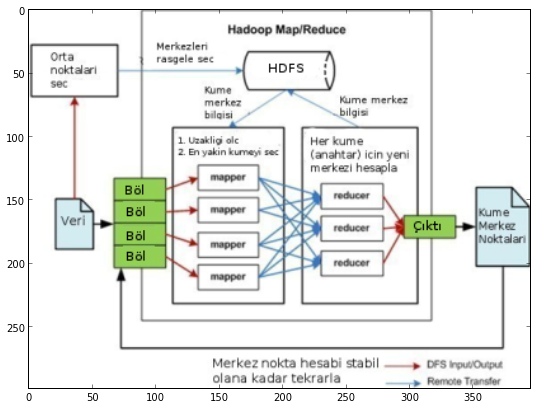
\includegraphics[width=0.7\textwidth]{kmeans_files/kmeans_fig_00.png}
\par
\end{center}
\end{codeoutput}
\end{codecell}
Simdi Hadoop ile ilgili bazi lojistik konulara gelelim:

Eger esleme safhasinda her nokta icin en yakin kumeyi bulmak istiyorsak,
o zaman (ilk basta rasgele bile olsa) kume merkezlerinin bilgisi tum
makinalarin erisebilecegi bir yerde olmali. Biz bu veriyi, centers.csv
adli dosyayi HDFS uzerinde tutmaya karar verdik, dosya ismi -archives
ile Hadoop'a gecilecek ve bu sekilde gecilen dosya isimlerine isleyen
script ile ayni dizindeymis gibi erisilebilir.

Paralel K-Means icin tek bir esle-indirge isletimi yeterli degil, bu
algoritma dongulu / ozyineli (iterative) bir algoritma, 5,10,20 kez
islemesi gerekebilir. Her dongu (indirgeme) sonunda yeni kume merkezleri
hesaplanacak, bu merkezler eski centers.csv yerini alacak ve islem
tekrar baslayacak.

Dongu sonundaki merkez bilgisi indirgeyicinin ciktisidir ve bu cikti
output/part-00000 dosyasi icinde. Unutmayalim, indirgeyicinin ciktisi
demek, tum indirgeyici makinalardan gelen anahtarlarin (ozetleme
ardindan) birlestirilmesi sonrasinda demek.

Simdi ham veriyi gosterelim, ve Hadoop'u baslatalim.

\begin{codecell}
\begin{codeinput}
\begin{lstlisting}
from pandas import *
df1 = read_csv("synthetic.txt",sep="   ")
plt.scatter(df1.ix[:,0],df1.ix[:,1])

\end{lstlisting}
\end{codeinput}
\begin{codeoutput}
\begin{verbatim}
<matplotlib.collections.PathCollection at 0xa4f23cc>
\end{verbatim}
\begin{center}
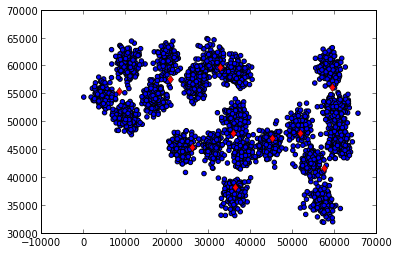
\includegraphics[width=0.7\textwidth]{kmeans_files/kmeans_fig_01.png}
\par
\end{center}
\end{codeoutput}
\end{codecell}
\begin{codecell}
\begin{codeinput}
\begin{lstlisting}

!ssh localhost -l hduser /home/hduser/Downloads/hadoop*/bin/stop-all.sh
!ssh localhost -l hduser /home/hduser/Downloads/hadoop*/bin/start-all.sh

\end{lstlisting}
\end{codeinput}
\begin{codeoutput}
\begin{verbatim}
no jobtracker to stop
\end{verbatim}
\begin{verbatim}
localhost: no tasktracker to stop
\end{verbatim}
\begin{verbatim}
no namenode to stop
\end{verbatim}
\begin{verbatim}
localhost: no datanode to stop
\end{verbatim}
\begin{verbatim}
localhost: no secondarynamenode to stop
\end{verbatim}
\begin{verbatim}
starting namenode, logging to /home/hduser/Downloads/hadoop-1.0.4/libexec/../logs/hadoop-hduser-namenode-burak-Aspire-S3.out
\end{verbatim}
\begin{verbatim}
localhost: starting datanode, logging to /home/hduser/Downloads/hadoop-1.0.4/libexec/../logs/hadoop-hduser-datanode-burak-Aspire-S3.out
\end{verbatim}
\begin{verbatim}
localhost: starting secondarynamenode, logging to /home/hduser/Downloads/hadoop-1.0.4/libexec/../logs/hadoop-hduser-secondarynamenode-burak-Aspire-S3.out
\end{verbatim}
\begin{verbatim}
starting jobtracker, logging to /home/hduser/Downloads/hadoop-1.0.4/libexec/../logs/hadoop-hduser-jobtracker-burak-Aspire-S3.out
\end{verbatim}
\begin{verbatim}
localhost: starting tasktracker, logging to /home/hduser/Downloads/hadoop-1.0.4/libexec/../logs/hadoop-hduser-tasktracker-burak-Aspire-S3.out
\end{verbatim}
\end{codeoutput}
\end{codecell}
Gerekli merkez verisinin tutulacagi yer /tmp demistik. Bu ismi ozellikle
sectik cunku hem yerel, komut satirindan (Hadoop olmadan) calisirken
rahat kullanilabilecek bir dizin olsun istedik. Bu dizini HDFS uzerinde
yaratalim (unutmayalim, HDFS demek ayri bir alem demek, pur Unix
komutlarimiz bile oraya erisemiyor)

\begin{codecell}
\begin{codeinput}
\begin{lstlisting}
!ssh localhost -l hduser /home/hduser/Downloads/hadoop*/bin/hadoop dfs -copyFromLocal $HOME/Documents/classnotes/stat/stat_hadoop_kmeans/synthetic.txt /user/hduser
\end{lstlisting}
\end{codeinput}
\begin{codeoutput}
\begin{verbatim}
copyFromLocal: Target /user/hduser/synthetic.txt already exists
\end{verbatim}
\end{codeoutput}
\end{codecell}
\begin{codecell}
\begin{codeinput}
\begin{lstlisting}
print open("mapper.py").read()
\end{lstlisting}
\end{codeinput}
\begin{codeoutput}
\begin{verbatim}
#!/usr/bin/python
import os,sys,itertools
import numpy as np
from numpy import linalg as la
os.environ['MPLCONFIGDIR']='/tmp' 
import pandas as pd

centers = pd.read_csv("centers.csv",header=None,sep=",")

def dist(vect,x):
    return np.fromiter(itertools.imap(np.linalg.norm, vect-x),dtype=np.float)

def closest(x):
    d = dist(np.array(centers)[:,1:3],np.array(x))
    return np.argmin(d)

comb = lambda x: str(x[0])+":"+str(x[1])

df = pd.read_csv(sys.stdin,header=None,sep="   ")
df['cluster'] = df.apply(closest,axis=1)
df['coord'] = df.apply(comb,axis=1)
df.to_csv(sys.stdout, sep='\t',index=False, cols=['cluster','coord'],
          header=None)
\end{verbatim}
\end{codeoutput}
\end{codecell}
Ustte comb ile kordinat verisini birlestirerek tek kolon haline
getirdik, cunku anahtar deger formunda veri uretmemiz gerekiyor, ve TAB
ayraci sadece tek anahtar ve tek deger ayrimi yapabilir, ve sadece bir
tane ayrac olabilir. Bu sebeple iki boyutlu veri oldugu icin iki sayi
olan deger, yani kordinat : uzerinden birlestirilerek tek bir deger
haline getirildi. Tabii indirgeci bu veriyi alinca bu islemin tersini
yapmasi lazim.

\begin{codecell}
\begin{codeinput}
\begin{lstlisting}
print open("reducer.py").read()
\end{lstlisting}
\end{codeinput}
\begin{codeoutput}
\begin{verbatim}
#!/usr/bin/python
import os,sys,itertools
import numpy as np
from numpy import linalg as la
os.environ['MPLCONFIGDIR']='/tmp' 
import pandas as pd

def coords(x):
    return pd.Series(np.array(str(x).split(":"),dtype=np.float64))

df = pd.read_csv(sys.stdin,sep="\t",names=['cluster','coord'])
df2 = df['coord'].apply(coords)
df3 = df.combine_first(df2)
df4 = df3.groupby('cluster').mean()
df4.to_csv(sys.stdout, sep=',',header=None)
\end{verbatim}
\end{codeoutput}
\end{codecell}
Alttaki blokta merkezleri rasgele veri noktalari uzerinden seciyoruz,
yani veri icinden rasgele 15 tane (k kadar) nokta cekip cikartik, onlari
baslangic merkezi yaptik. Bu salt rasgele sayi uretimi ile de
yapilabilirdi.

Komut satirindan tek makina icin Hadoop'suz isletelim,

\begin{codecell}
\begin{codeinput}
\begin{lstlisting}
import os,sys,itertools
from numpy import linalg as la
import pandas as pd
k = 15
df = read_csv("synthetic.txt",header=None,sep="   ")
centers = df.take(np.random.permutation(len(df))[:k])
centers.to_csv("centers.csv",header=None)
for i in range(20):
    os.system("cat synthetic.txt | python mapper.py | python reducer.py > centers2.csv")
    os.system("cp centers2.csv centers.csv")
    os.system("cp centers2.csv /tmp/centers-local-%i.csv" % i)

\end{lstlisting}
\end{codeinput}
\end{codecell}
\begin{codecell}
\begin{codeinput}
\begin{lstlisting}
i = 19
df1 = read_csv("synthetic.txt",sep="   ")
plt.scatter(df1.ix[:,0],df1.ix[:,1])
plt.hold(True)
df2 = read_csv("/tmp/centers-local-%d.csv" % i,header=None,index_col=0)
plt.plot(df2.ix[:,1],df2.ix[:,2],'rd')

\end{lstlisting}
\end{codeinput}
\begin{codeoutput}
\begin{verbatim}
[<matplotlib.lines.Line2D at 0xa9657cc>]
\end{verbatim}
\begin{center}
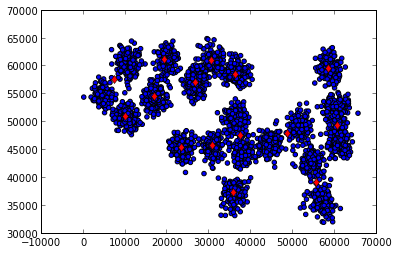
\includegraphics[width=0.7\textwidth]{kmeans_files/kmeans_fig_02.png}
\par
\end{center}
\end{codeoutput}
\end{codecell}
Simdi K-Means'i Hadoop'tan isleten kosturucu (runner) program. Bu
program esleme, indirgeme safhalarini cagiracak, ve indirgeyici sonrasi
ciktiyi alip yeni kume merkezi yapacak, bunun gibi idari / temizlik
islerini halledecek.

\begin{codecell}
\begin{codeinput}
\begin{lstlisting}
import os
os.system("cp mapper.py /tmp/")
os.system("chmod a+r /tmp/mapper.py")
os.system("chmod a+x /tmp/mapper.py")

os.system("cp reducer.py /tmp/")
os.system("chmod a+r /tmp/reducer.py")
os.system("chmod a+x /tmp/reducer.py")

k = 15
df = read_csv("synthetic.txt",header=None,sep="   ")
centers = df.take(np.random.permutation(len(df))[:k])
os.system("rm /tmp/centers.csv")
os.system("ssh localhost -l hduser rm /tmp/centers.csv")
centers.to_csv("/tmp/centers.csv",header=None)

hp_cmd = "ssh localhost -l hduser /home/hduser/Downloads/hadoop*/bin/hadoop"
streaming_cmd = "/home/hduser/Downloads/hadoop*/contrib/streaming/hadoop-*streaming*.jar"
os.system("ssh localhost -l hduser rm /tmp/centers-*-out.csv")

for i in range(20):
    os.system("%s dfs -rmr /user/hduser/output" % hp_cmd)
    os.system("%s jar %s -files /tmp/centers.csv -input synthetic.txt -output output -mapper /tmp/mapper.py -reducer /tmp/reducer.py -numReduceTasks 1" % (hp_cmd,streaming_cmd))
    os.system("%s dfs -copyToLocal /user/hduser/output/part-00000 /tmp/centers-%d-out.csv" % (hp_cmd,i) )
    os.system("ssh localhost -l hduser rm /tmp/centers.csv")
    os.system("rm /tmp/centers.csv")
    os.system("%s dfs -copyToLocal /user/hduser/output/part-00000 /tmp/centers.csv" % (hp_cmd) )

\end{lstlisting}
\end{codeinput}
\end{codecell}
Ustte K-Means'i 20 kere islettigimizi goruyoruz. Eger istenirse (hatta
daha iyi olur) dongu bir while icine konur ve bitis icin ``stabilite
sarti'' aranir. Stabilite yeni kume merkezinin eskisinden ``cok fazla
degisik olup olmadigi'' sartidir, degisim yoksa artik sonucu bulmusuz
demektir, daha fazla donguye gerek kalmayacaktir. Biz donguyu 20 kere
donguyu islettik, (bu problem icin) yeterli oldu.

K-Means isini bitirdikten sonra elde edilen sonuclari artik HDFS'ten
yerel dizinimize alabiliriz. Nihai kume merkezleri /tmp/centers-..
icinde. Bu merkezleri alip, ham veri uzerinde kirmizi nokta olarak
gosteriyoruz.

\begin{codecell}
\begin{codeinput}
\begin{lstlisting}
i = 19
df1 = read_csv("synthetic.txt",sep="   ")
plt.scatter(df1.ix[:,0],df1.ix[:,1])
plt.hold(True)
df2 = read_csv("/tmp/centers-%d-out.csv" % i,header=None,index_col=0)
plt.plot(df2.ix[:,1],df2.ix[:,2],'rd')
\end{lstlisting}
\end{codeinput}
\begin{codeoutput}
\begin{verbatim}
[<matplotlib.lines.Line2D at 0xa6a5aec>]
\end{verbatim}
\begin{center}
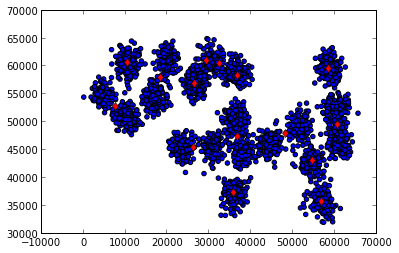
\includegraphics[width=0.7\textwidth]{kmeans_files/kmeans_fig_03.png}
\par
\end{center}
\end{codeoutput}
\end{codecell}
Sonuclar fena degil. Iste bu metotla terabayt olceginde, devasa bir
veriyi 20-30 makinaya dagitarak parca parca isleyip kumelemeniz
mumkundur. Endustride son zamanlarda habire duyulan Buyuk Veri (Big
Data) olayi iste bu.

\end{document}
